\documentclass[crop,tikz]{standalone}

\usepackage{pgfplots}
\pgfplotsset{compat=1.16}
 
\begin{document}
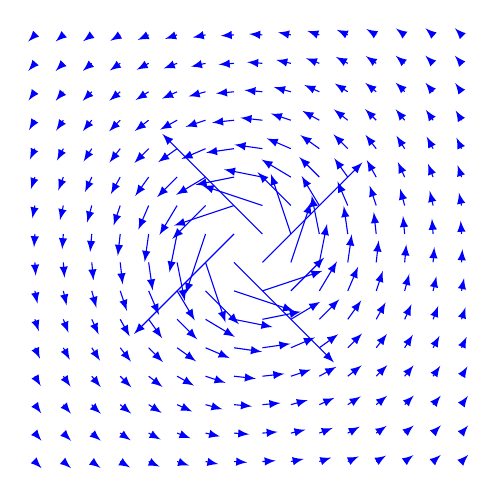
\begin{tikzpicture}
\begin{axis}[
  xmin = -2, xmax = 2,
  ymin = -2, ymax = 2,
  zmin = 0, zmax = 1,
  axis equal image,
  height=7cm,
  view = {0}{90},
  color=blue,
  xtick={\empty},
  ytick={\empty},
  hide axis,
  samples = 16,
  clip=false,
  ]
  \addplot3[
    point meta = {sqrt(x^2+y^2)},
    quiver = {
      u = {-y/(x^2+y^2)},
      v = {x/(x^2+y^2)},
      scale arrows = 0.25,
      every arrow/.append style={
        -{latex[scale={max(0.7,\pgfplotspointmetatransformed/1000)}]},
      },
   },
   domain = -2:2,
   domain y = -2:2,
  ] {0};
\end{axis}
\end{tikzpicture}
\end{document}
